\documentclass[12pt,a4letter]{article}
\usepackage[T2A]{fontenc}
\usepackage[utf8]{inputenc}
\usepackage[russian]{babel}
\usepackage{graphicx}
\usepackage{amsfonts}
\usepackage{indentfirst}
\usepackage{amsmath}
\usepackage{amsthm}
\usepackage{nicematrix}
\usepackage{hyperref}
\hypersetup{
    colorlinks=true,
    linkcolor=black,
    filecolor=magenta,      
    urlcolor=cyan,
    pdftitle={Lab3},
    pdfpagemode=FullScreen,
}
\usepackage{soulutf8}
\usepackage[left=1cm,right=1cm,
    top=2cm,bottom=2cm]{geometry}
\usepackage{titleps}
    \newpagestyle{main}{
        \setheadrule{0.4pt}
        \sethead{something}{\thepage}{}
}
%\pagestyle{main}
\theoremstyle{plain}
\newtheorem{theorem}{Теорема}[section]
\newtheorem{corollary}{Следствие}[theorem]
\newtheorem*{example}{\textit{Пример}}
\newtheorem*{definition}{Определение}
\begin{document}
\begin{titlepage}
    \newpage
    \begin{center}
    \begin{tabular}{cc}
         \parbox{12cm}{\centering \textbf{НИУ ИТМО}} & \parbox{4cm}{\includegraphics[width=4cm]{itmo3}}\\
         \\
         \hline
         \hline
    \end{tabular}
    \end{center}
    
    \begin{center}
    \caps{\textbf{Факультет систем управления и робототехники}}\\ 
    \end{center}
    
    \vspace{1cm}
    
    \begin{center}
        \textsc{Лабораторная работа №2 \\ по дисциплине <<Техническое зрение>>}
    \end{center}
    
    \vspace{8em}
    
    \noindent Выполнил:  \hfill Гридусов Денис
    
    \vspace{20pt}
    
    \noindent Преподаватель: \hfill Шаветов С.В. \\
    \\
    \vfill
    
    \begin{center}
    Санкт-Петербург \\2024 г.
    \end{center}
    
    \end{titlepage}
    
    \tableofcontents
    \newpage
    \section{Введение}
    \noindent \textbf{Цель работы:} освоить основные виды отображений и использовать геометрические преобразования для решения задач пространственной коррекции изображений.
    \\
    \noindent \textbf{Код: } \href{https://github.com/D2J3D/Lab_CV}{github}
    \newpage
    \section{Простейшие геометрические преобразования}
    Возьмем произвольное изображение, например:
    \begin{figure}[h]
        \centering
        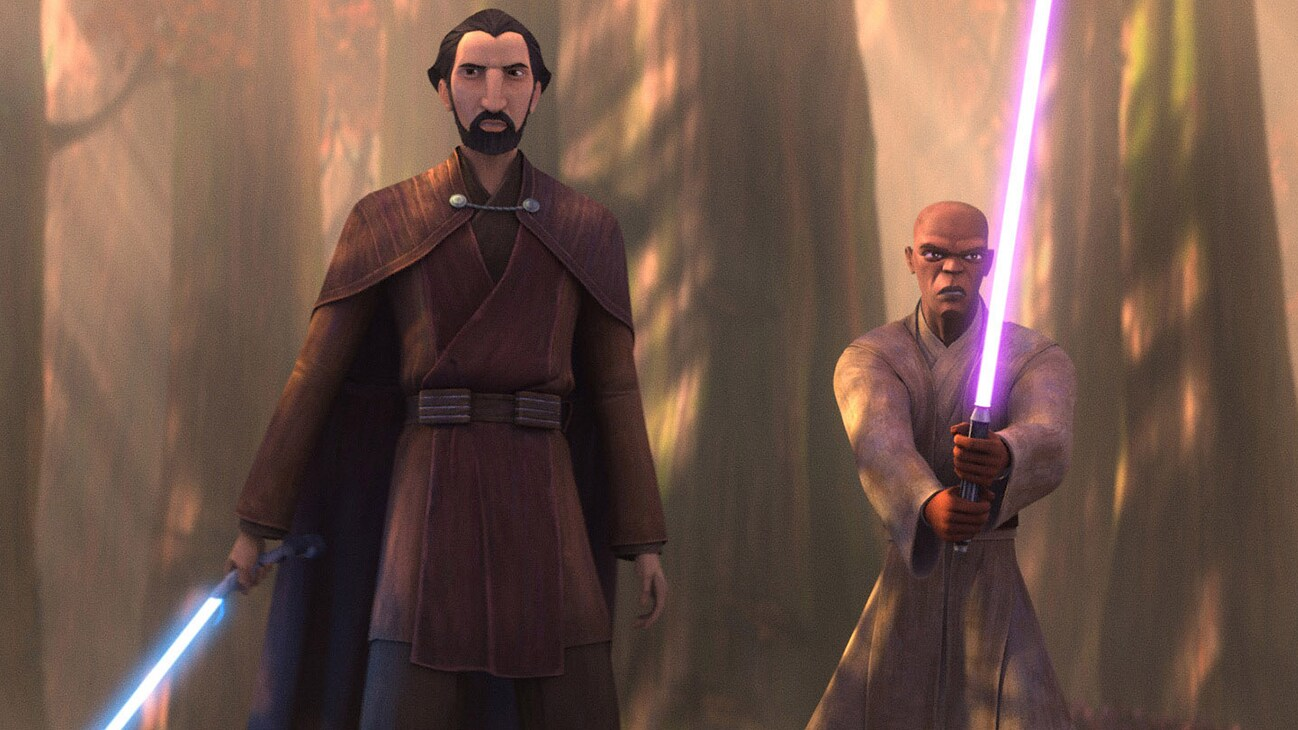
\includegraphics[scale=0.3]{"../images/original/g_disney_talesofthejedi_870_05_47cd6d1c.jpeg"}
        \caption{Исходное изображение}
    \end{figure}
    \\
    \subsection{Сдвиг изображения}
    \noindent Для разминки применим самое очевидное геометрическоео преобразование - сдивг изоюбражения.
    Матрица отображения $T$ выглядит следующим образом:
    \begin{center}
        $
        T = 
        \begin{bmatrix}
            1 & 0 & 0\\
            0 & 1 & 0\\
            C & F & 1 
        \end{bmatrix}
        $,
    \end{center}
    где $F$ - величина сдвига по оси $Oy$, а $C$ - величина сдвига по оси $Ox$.
    \\
    \noindent \textbf{Листинг 2.1} Сдвиг изображения
    \begin{lstlisting}
    cv::Mat img_shift(cv::Mat img, int x_hist, int y_hist) {
        cv::Mat T = (cv::Mat_ <double>(2, 3) << 1, 0, x_hist, 0, 1, y_hist);
        cv::Mat img_shift;
        cv::warpAffine(img, img_shift, T, cv::Size(img.cols, img.rows));
        return img_shift;
    }
    \end{lstlisting}  
    \begin{figure}[h]
        \centering
        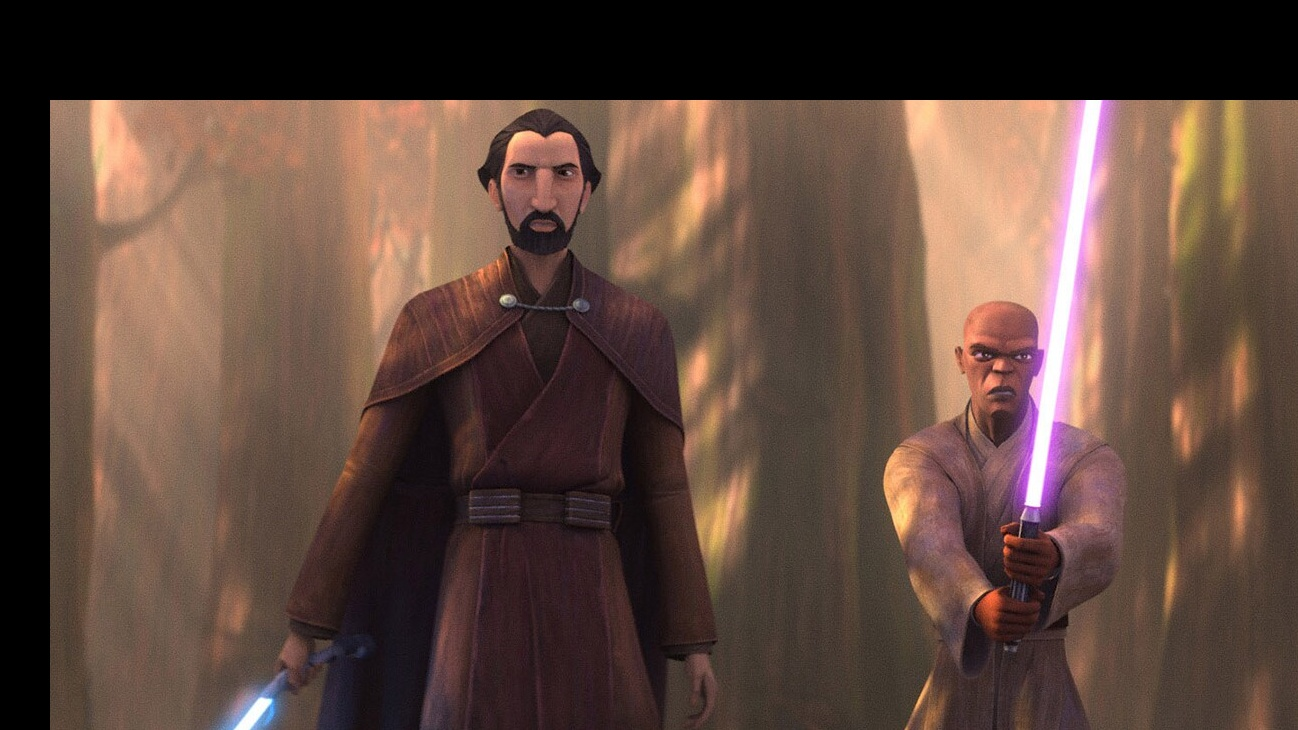
\includegraphics[scale=0.3]{"../images/results/shift_img.jpg"}
        \caption{Сдвиг изображения на 50 пикселей по оси X, 100 по Y}
    \end{figure}
    \newpage
    \subsection{Отражение изображения}
    Отразим изображение, относительно оси Ox, матрица преобразования:
    \begin{center}
        $
        T = 
        \begin{bmatrix}
            1 & 0 & 0\\
            0 & -1 & 0\\
            0 & 0 & 1
        \end{bmatrix}
        $
    \end{center}
    \noindent \textbf{Листинг 2.2} Отражение относительно оси $Ox$
    \begin{lstlisting}
cv::Mat img_reflection(cv::Mat img) {
    cv::Mat T = (cv::Mat_ <double>(2, 3) << 1, 0, 0, 0, -1, img.rows - 1);
    cv::Mat img_reflected;
    cv::warpAffine(img, img_reflected, T, cv::Size(img.cols, img.rows));
    return img_reflected;
}
    \end{lstlisting}
    \begin{figure}[h]
        \centering
        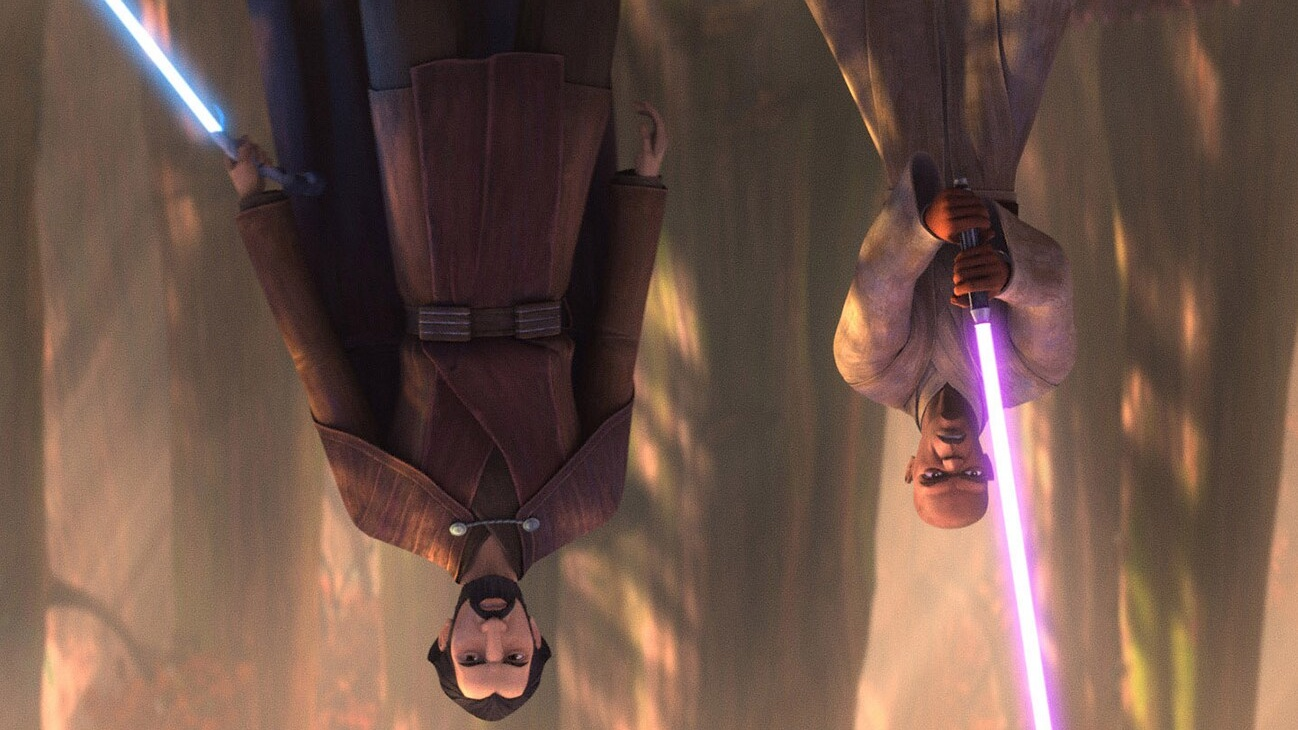
\includegraphics[scale=0.3]{"../images/results/img_reflection.jpg"}
        \caption{Отраженное относительно оси $Ox$ изображение}
    \end{figure}
    \newpage
    \subsection{Однородное масштабирование изображения}
    \noindent А теперь масштабируем изображение, матрица преобразования:
    \begin{center}
        $
        T = 
        \begin{bmatrix}
            \alpha & 0 & 0\\
            0 & \beta & 0\\
            0 & 0 & 1
        \end{bmatrix}
        $,
    \end{center}
    где $\alpha$ отвечает за расятжение по оси X, а $\beta$ - по оси Y.
    \\ \noindent \textbf{Листинг 2.3} Однородное ($\alpha = \beta$) растяжение изображения
    \begin{lstlisting}
cv::Mat uniform_resize(cv::Mat img, double coeff) {
    cv::Mat T = (cv::Mat_ <double>(2, 3) << coeff, 0, 0, 0, coeff, 0);
    cv::Mat img_resized;
    cv::warpAffine(img, img_resized, T, cv::Size(int(img.cols * coeff), int(img.rows * coeff)));
    return img_resized;
} 
    \end{lstlisting}

    \subsection{Поворот изображения}
    Повернем изображение на произвольный угол $\varphi$, матрица преобразования:
    \begin{center}
        $
        T = 
        \begin{bmatrix}
            \cos \varphi & \sin \varphi & 0\\
            -\sin \varphi & \cos \varphi & 0\\
            0 & 0 & 1
        \end{bmatrix}
        $  
    \end{center}
    \noindent \textbf{Листинг 2.4} Поворот на произвольный угол $\varphi$
    \begin{lstlisting}
cv::Mat img_rotate(cv::Mat img, double phi) {
    double r_phi = phi * M_PI / 180.0;
    cv::Mat T = (cv::Mat_ <double>(2, 3) << std::cos(r_phi), -std::sin(r_phi), 0, std::sin(r_phi), std::cos(r_phi), 0);
    cv::Mat img_rotated;
    cv::warpAffine(img, img_rotated, T, cv::Size(img.cols, img.rows));
    return img_rotated;
}
    \end{lstlisting}
    \begin{figure}[h]
        \centering
        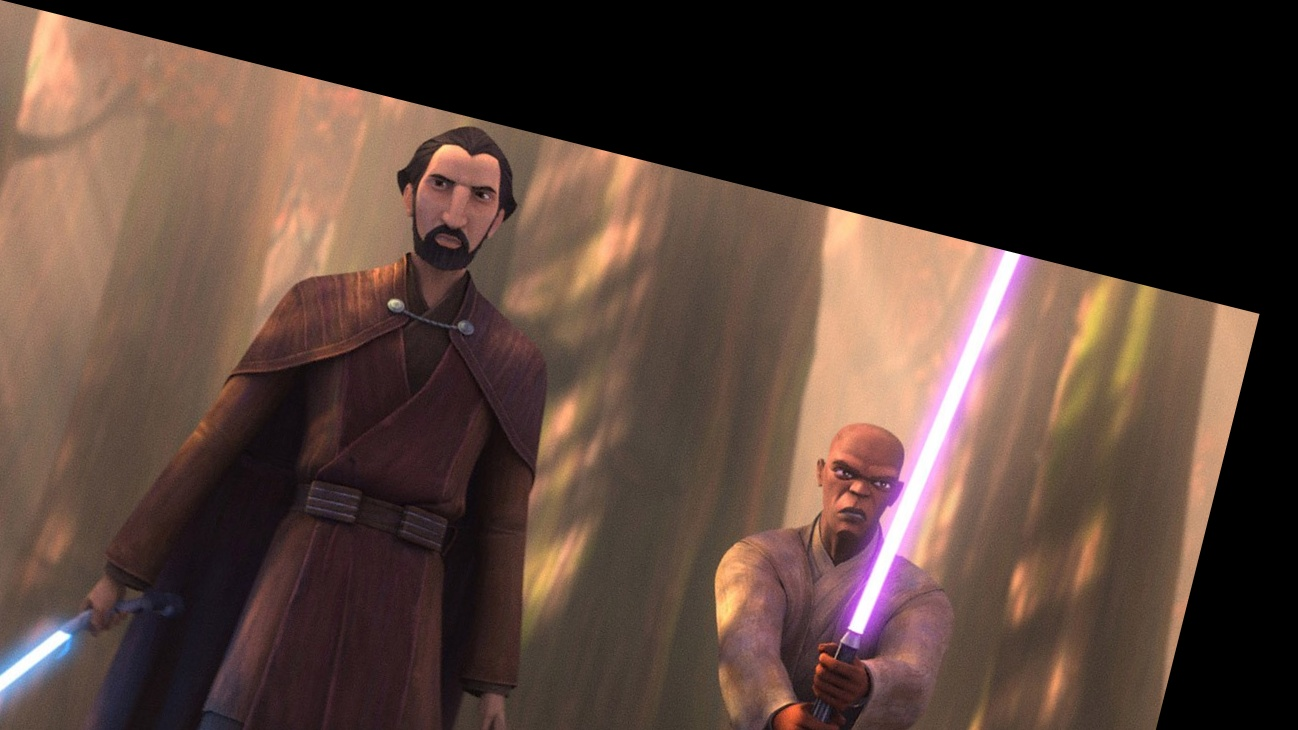
\includegraphics[scale=0.26]{"../images/results/img_rotation.jpg"}
        \caption{Поворот на 14 градусов вокруг левого верхнего угла}
    \end{figure}
    \newpage
    \subsection{Поворот вокруг центра изображения}
    Попробуем теперь повернуть изображение вокруг его центра, для этого 
    нужно лишь сдвинуть центр в левый верхний угол, повернуть как в предыдущем пункте и потом сдвинуть центр на прежнее место. Матрица преобразования $T$ выглядеть будет так:
    \begin{center}
        $
        T =
        \begin{bmatrix}
            1 & 0 & -\frac{img.cols - 1}{2}\\
            0 & 1 & -\frac{img.rows - 1}{2}
            \\0 & 0 & 1
        \end{bmatrix}
        \
        \times
        \begin{bmatrix}
            \cos \varphi & \sin \varphi & 0\\
            -\sin \varphi & \cos \varphi & 0\\
            0 & 0 & 1
        \end{bmatrix}
        \times
        \begin{bmatrix}
            1 & 0 & \frac{img.cols - 1}{2}\\
            0 & 1 & \frac{img.rows - 1}{2}\\
            0 & 0 & 1
        \end{bmatrix}
        $
    \end{center}
    \noindent \textbf{Листинг 2.5} Поворот вокруг центра на произвольный угол $\varphi$
    \begin{lstlisting}
cv::Mat img_centered_rotate(cv::Mat img, double phi) {
    double r_phi = phi * M_PI / 180.0;
    cv::Mat T2 = (cv::Mat_ <double>(3, 3) << std::cos(r_phi), -std::sin(r_phi), 0, std::sin(r_phi), std::cos(r_phi), 0, 0, 0, 1);
    cv::Mat T1 = (cv::Mat_ <double>(3, 3) << 1, 0, -(img.rows - 1) / 2.0, 0, 1, -(img.cols - 1) / 2.0, 0, 0, 1);
    cv::Mat T3 = (cv::Mat_ <double>(3, 3) << 1, 0, (img.rows - 1) / 2.0, 0, 1, (img.cols - 1) / 2.0, 0, 0, 1);

    cv::Mat T = cv::Mat(T3 * T2 * T1, cv::Rect(0, 0, 3, 2));
    cv::Mat img_rotated;
    cv::warpAffine(img, img_rotated, T, cv::Size(img.cols, img.rows));
    return img_rotated;
}

    \end{lstlisting}
    \begin{figure}[h]
        \centering
        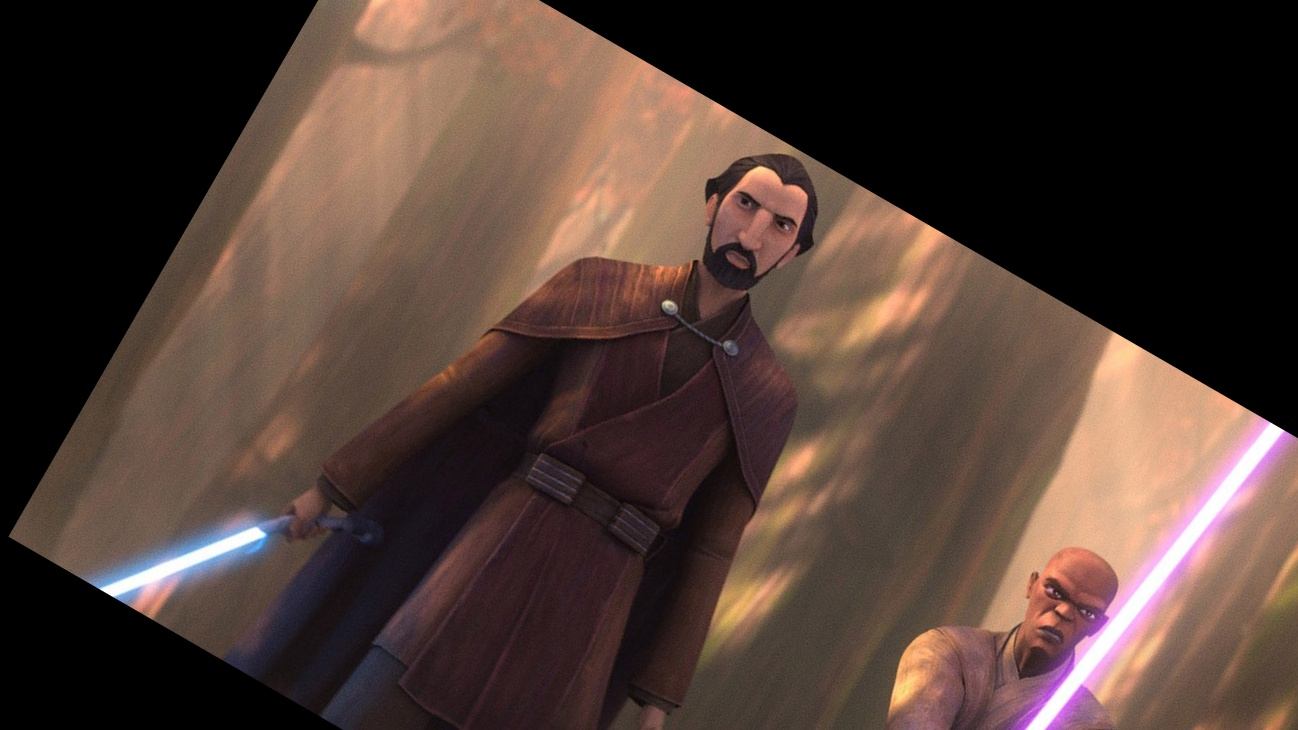
\includegraphics[scale=0.3]{"../images/results/img_center_rotation.jpg"}
        \caption{Поворот на 30 градусов вокруг центра изображения}
    \end{figure}
    \subsection{Аффинное отображение}
   \noindent Аффинное отображение — это отображение, при котором
параллельные прямые переходят в параллельные прямые, пересекающиеся в пересекающиеся, скрещивающиеся в скрещивающиеся; сохраняются отношения длин отрезков, лежащих на одной прямой (или на параллельных прямых), и отношения площадей фигур.\\
\\ \noindent \textbf{Листинг 2.6} Аффинное преобразование
\begin{lstlisting}
cv::Mat affine_resize(cv::Mat img) {
    std::vector <cv::Point2f> ptr_src = { {50, 100}, {350, 100}, {50, 400} };
    std::vector <cv::Point2f> ptr_dst = { {50, 150},{200, 150},{100, 400} };

    cv::Mat T = cv::getAffineTransform(ptr_src, ptr_dst);
    cv::Mat img_resized;
    cv::warpAffine(img, img_resized, T, cv::Size(img.cols, img.rows));

    return img_resized;
}
\end{lstlisting}
\begin{figure}[h]
    \centering
    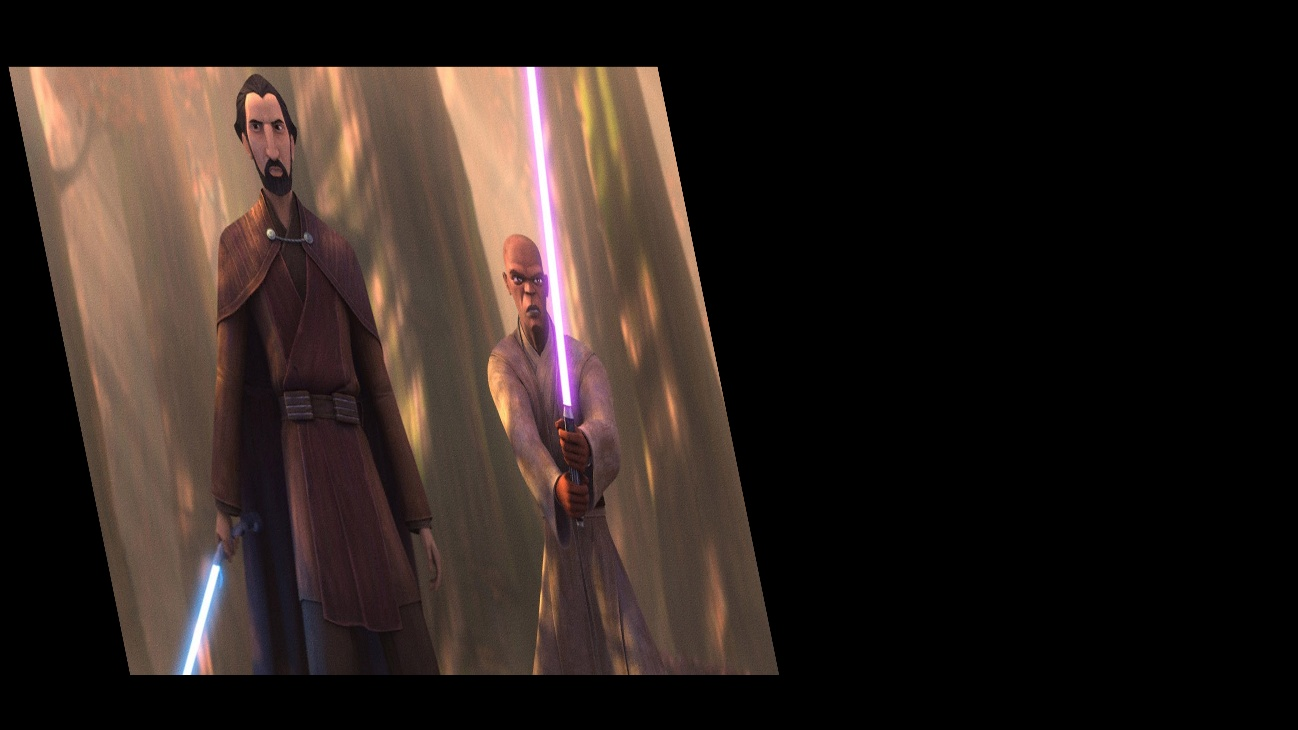
\includegraphics[scale=0.3]{"../images/results/affine_resize.jpg"}
    \caption{Аффинное преобразование изображения}
\end{figure}
\subsection{Скос изображения}
Запишем матрицу отображения:
\begin{center}
    $T = 
    \begin{bmatrix}
        1 & 0 & 0\\
        s & 1 & 0\\
        0 & 0 & 1
    \end{bmatrix}
    $
\end{center}
\noindent \textbf{Листинг 2.7} Скос изображения
\begin{lstlisting}
cv::Mat img_bevel(cv::Mat img, double s) {
        cv::Mat T = (cv::Mat_ <double>(2, 3) << 1, s, 0, 0, 1, 0);
        cv::Mat img_bevel;
        cv::warpAffine(img, img_bevel, T, cv::Size(img.cols, img.rows));
        return img_bevel;
    } 
\end{lstlisting}
\begin{figure}[h]
    \centering
    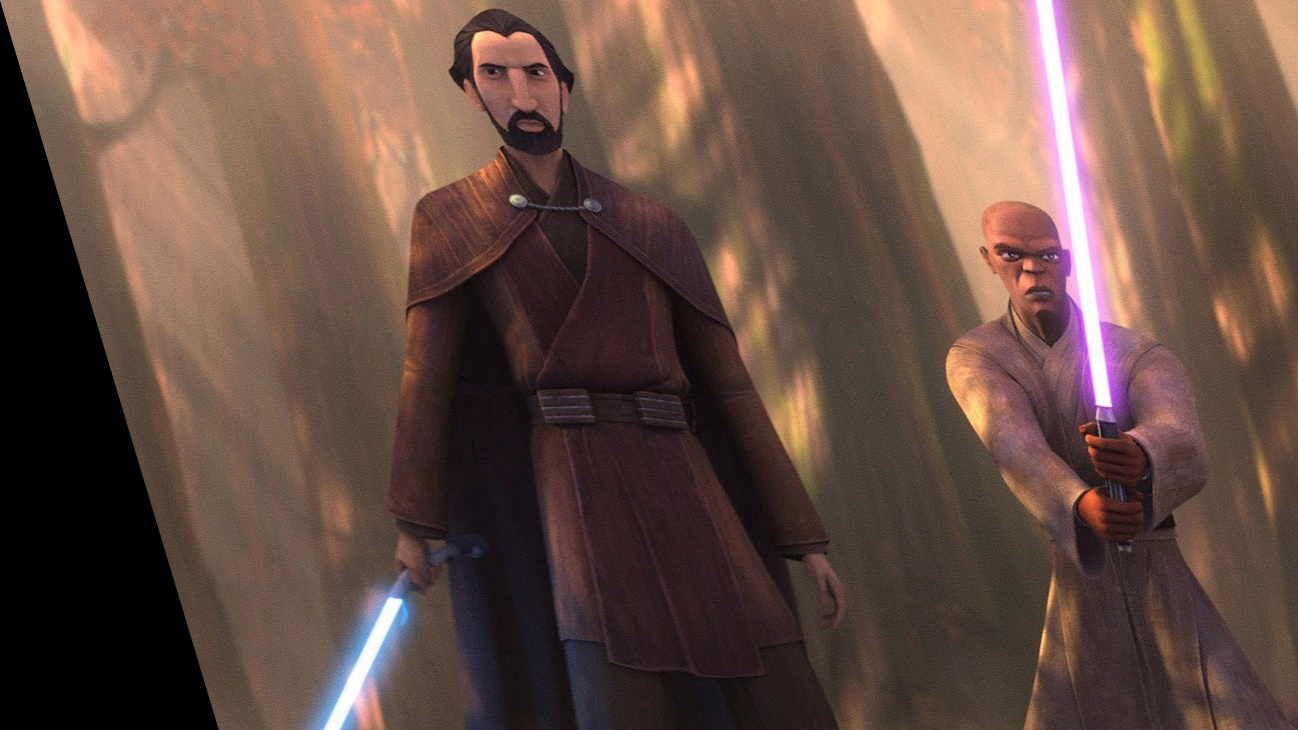
\includegraphics[scale=0.3]{"../images/results/img_bevel.jpg"}
    \caption{Скос изображения с s = 0.3}
\end{figure}
\newpage
\subsection{ Кусочно-линейные преобразование    }
Теперь применим преобразование не ко всему изображению, а только к его части (к ROI).
\\
\noindent \textbf{Листинг 2.8} Растяжение только правой части изображения в s раз 
\begin{lstlisting}
cv::Mat uniform_ROI_transform(cv::Mat img, double s) {
    cv::Mat T = (cv::Mat_ <double>(2, 3) << s, 0, 0, 0, 1, 0);
    cv::Mat img_piece_linear = img.clone();
    cv::Mat img_right = img_piece_linear(cv::Rect(int(img.cols / 2.0), 0, img.cols - int(img.cols / 2.0), img.rows));
    cv::warpAffine(img_right, img_right, T, cv::Size(img.cols - int(img.cols / 2.0), img.rows));
    return img_piece_linear;
}

\end{lstlisting}
\begin{figure}[h]
    \centering
    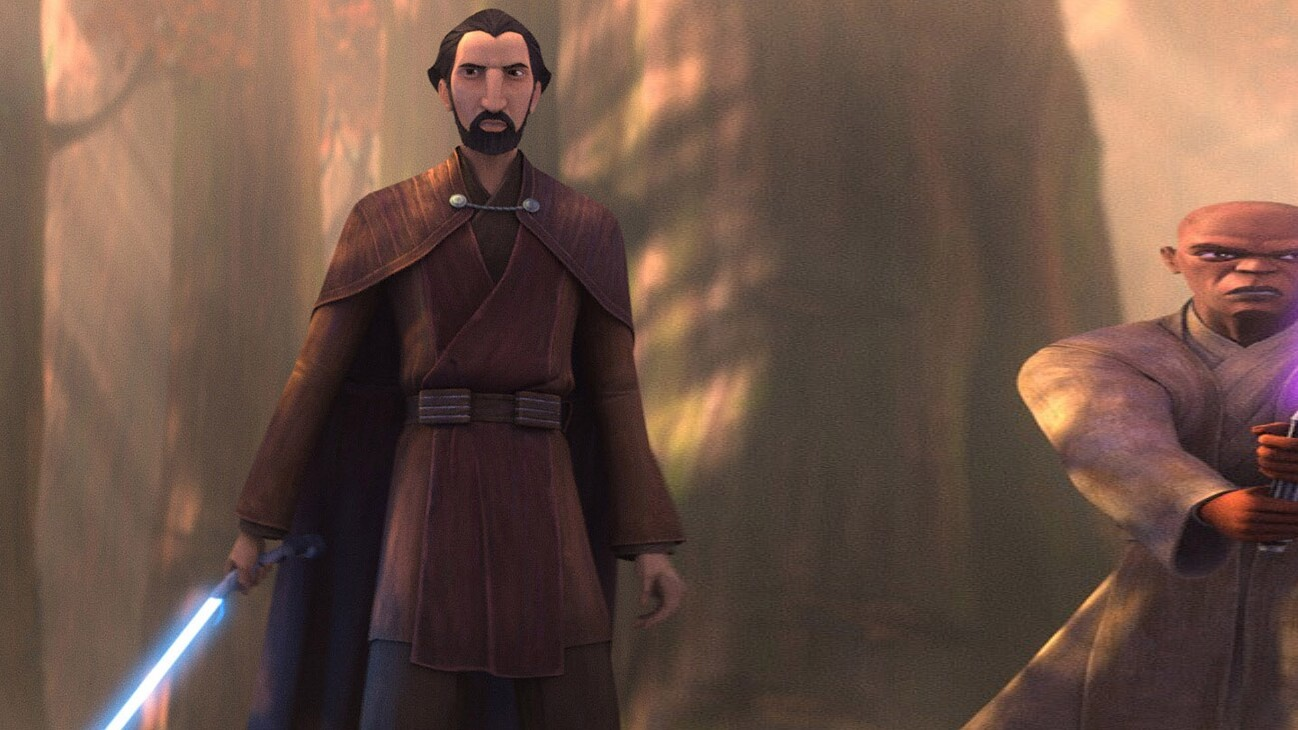
\includegraphics[scale=0.3]{"../images/results/roi_transformed_img.jpg"}
    \caption{Левая половина без изменений,  правая растягивается в 2 раза по оси X}
\end{figure}
\newpage
\subsection{Проекционное отображение}
\noindent Матрица T:
\begin{center}
    $
    T = 
    \begin{bmatrix}
        A & B & C\\
        D & E & F\\
        G & H & I
    \end{bmatrix}
    $
\end{center}
\noindent \textbf{Листинг 2.9} Проекционное отображение
\begin{lstlisting}
cv::Mat projective_transform(cv::Mat img, double params[9]) {
    // params[9] = A, B, C, D, E, F, G, I
    cv::Mat T = (cv::Mat_ <double>(3, 3) << params[0], params[1], params[2], params[3], params[4], params[5], params[6], params[7], params[8]);
    cv::Mat img_projective;
    cv::warpPerspective(img, img_projective, T, cv::Size(img.cols, img.rows));
    return img_projective;
}
\end{lstlisting}
\begin{figure}[h]
    \centering
    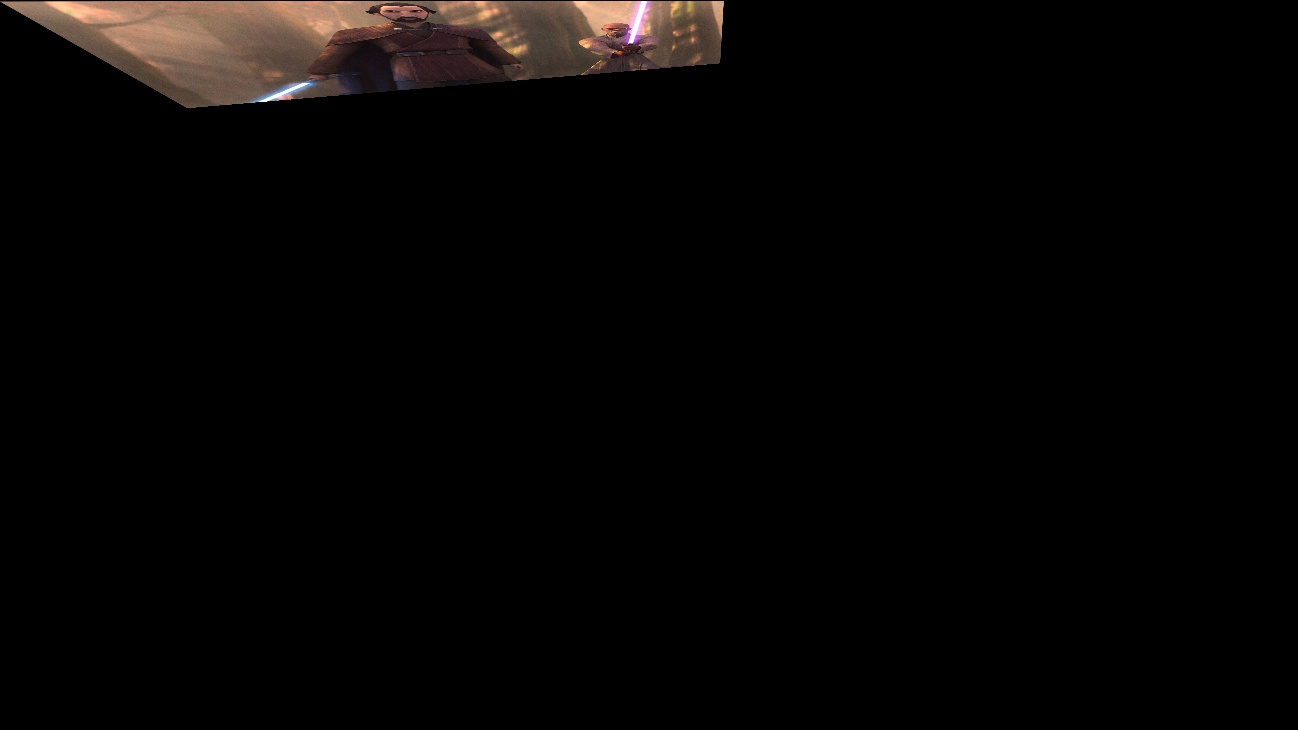
\includegraphics[scale=0.3]{"../images/results/projective_transformed_image.jpg"}
    \caption{Проекционное отображение}
\end{figure}

\subsection{Полиномиальное отображение}
Формула преобразования координат:
\begin{equation}
    \begin{cases}
        x^\prime = a_1 + a_2 x + a_3 y + a_4 x^2 + a_5 xy + a_6 y^2\\
        y^\prime = b_1 + b_2 x + b_3 y + b_4 x^2 + b_5 xy + b_6 y^2
    \end{cases}
\end{equation}
\noindent \textbf{Листинг 2.10} Полиномиальное преобразование
\begin{lstlisting}
cv::Mat polinomial_transformation(cv::Mat img, double T[2][6]) {
    cv::Mat img_polinomial;
    if (img.depth() == CV_8U) {
        img.convertTo(img_polinomial, CV_32F, 1.0 / 255);
    }
    else {
        img_polinomial = img;
    }
    std::vector<cv::Mat> img_BGR;
    cv::split(img_polinomial, img_BGR);

    for (int channel = 0; channel < img_BGR.size(); channel++) {
        img_polinomial = cv::Mat::zeros(img_BGR[channel].rows, img_BGR[channel].cols, img_BGR[channel].type());
        for (int x = 0; x < img_BGR[channel].cols; x++) {
            for (int y = 0; y < img_BGR[channel].rows; y++) {
                int xnew = int(round(T[0][0] + x * T[0][1] + y * T[0][2] + x * x * T[0][3] + x * y * T[0][4] + y * y * T[0][5]));
                int ynew = int(round(T[1][0] + x * T[1][1] + y * T[1][2] + x * x * T[1][3] + x * y * T[1][4] + y * y * T[1][5]));
                if ((xnew >= 0) && (xnew < img_BGR[channel].cols) && (ynew >= 0) && (ynew < img_BGR[channel].rows)) {
                    img_polinomial.at<float>(ynew, xnew) = img_BGR[channel].at<float>(y, x);
                }
            }
        }
        img_BGR[channel] = img_polinomial;
    }

    cv::merge(img_BGR, img_polinomial);
    if (img.depth() == CV_8U) {
        img_polinomial.convertTo(img_polinomial, CV_8U, 255);
    }

    return img_polinomial;
}
\end{lstlisting}
\begin{figure}[h]
    \centering
    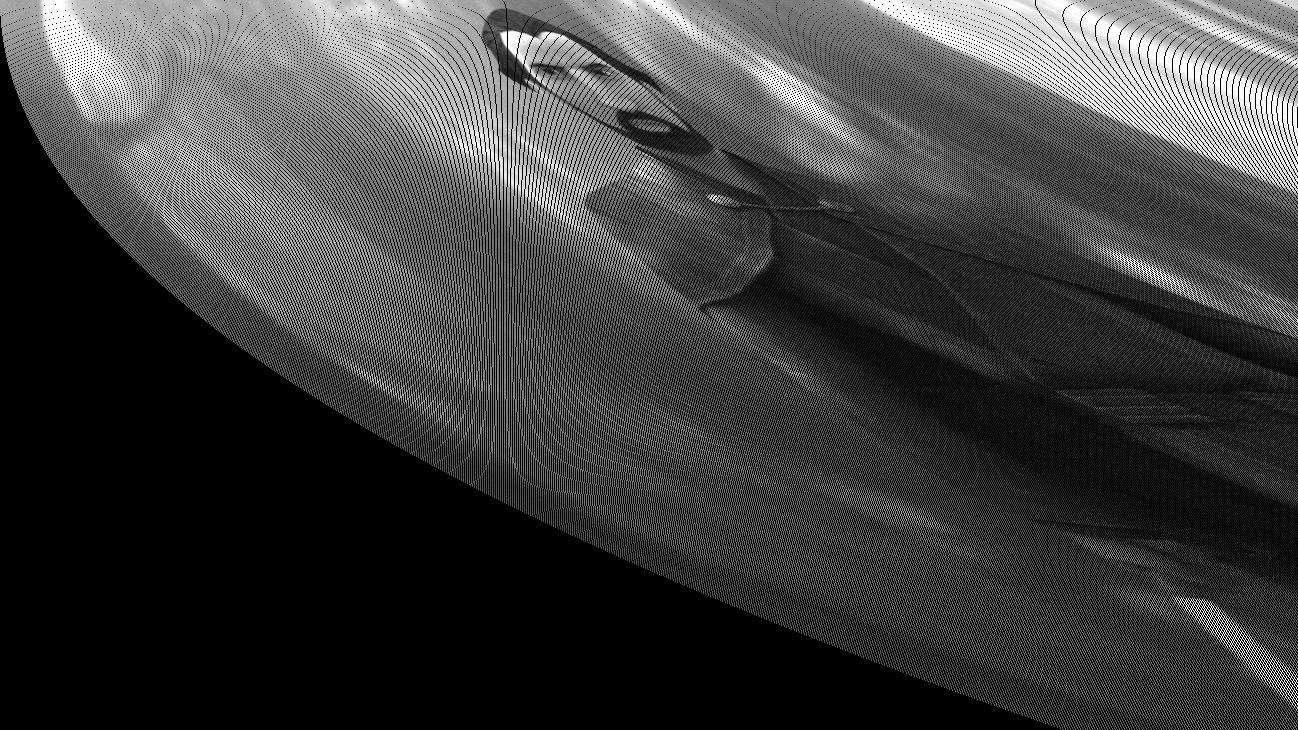
\includegraphics[scale=0.3]{"../images/results/polinomial_transformed_image.jpg"}
    \caption{Полиномиальное отображение}
\end{figure}
\newpage


\subsection{Синусоидальное искажение}
\noindent \textbf{Листинг 2.11} Синусоидальное искажение
\begin{lstlisting}
cv::Mat sin_transformation(cv::Mat img, double s) {
    cv::Mat u = cv::Mat::zeros(img.size(), CV_32F);
    cv::Mat v = cv::Mat::zeros(img.size(), CV_32F);
    for (int x = 0; x < img.cols; x++) {
        for (int y = 0; y < img.rows; y++) {
            u.at<float>(y, x) = float(x + s * std::sin(2 * M_PI * y / 90.0));
            v.at<float>(y, x) = float(y);
        }
    }
    cv::Mat sinusoid_image;
    cv::remap(img, sinusoid_image, u, v, cv::INTER_LINEAR);
    return sinusoid_image;
}

\end{lstlisting}
\begin{figure}[h]
    \centering
    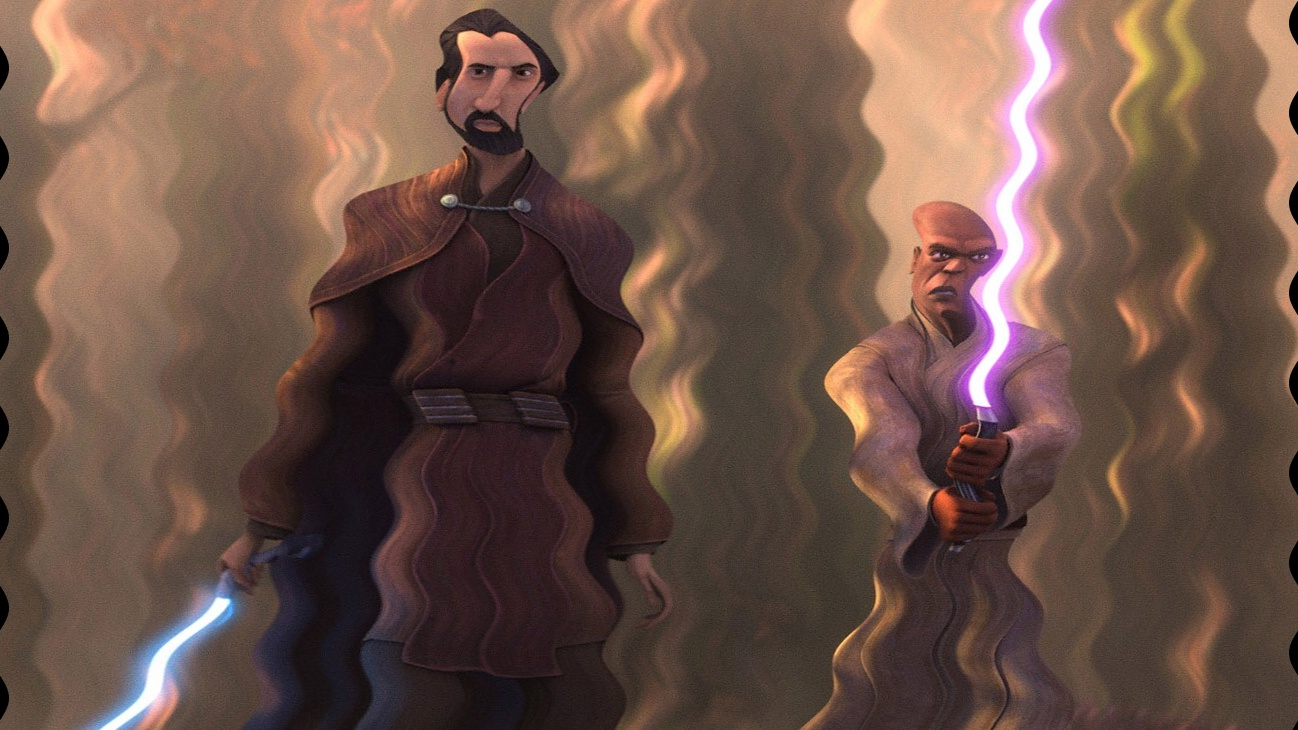
\includegraphics[scale=0.3]{"../images/results/sinusoidal_distortion_img.jpg"}
    \caption{Синусоидальное искажение s = 9}
\end{figure}

\newpage

\section{Коррекция дисторсии}
\noindent  Дисторсия — это оптическое искажение, выражающееся в искривлении прямых линий. 
Для корректного анализа изображения лучше снизить влияние дисторсии на геометрию изображения. Если у нас есть прямой доступ к камере, которую мы хотим откалибровать, то с помощью маркеров ArUco можно провести коррекцию дисторсии.
Если же доступа к камере у нас нет, можно попытаться исправить подушкообразную дисторсию наложением бочкообразной, а бочкообразную дисторсию - наложением подушкообразной. 
Приступим.\\
\begin{figure}[h]
    \centering 
    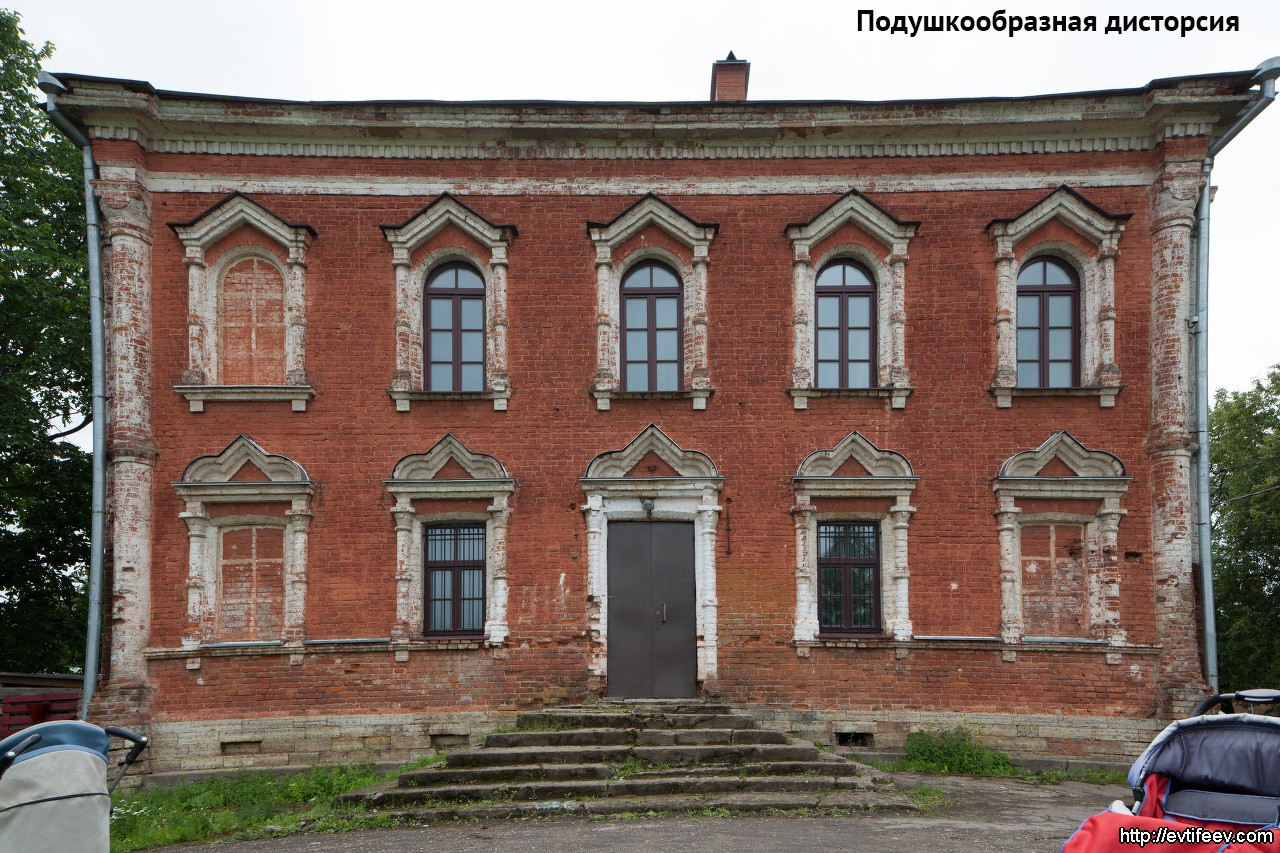
\includegraphics[scale=0.4]{../images/original/pd.jpg}
    \caption{Изображение с выраженной подушкообразной дисторсией}
\end{figure}

\clearpage
\noindent \textbf{Листинг 3.1} Наложение бочкообразной дисторсии
\begin{lstlisting}
cv::Mat barrel_distortion(cv::Mat img) {
    cv::Mat xi, yi;
    std::vector<float> t_x, t_y;
        for (int i = 0; i < img.cols; i++) {
        t_x.push_back(float(i));
    }
    for (int i = 0; i < img.rows; i++) {
        t_y.push_back(float(i));
    }
    
    cv::repeat(cv::Mat(t_x).reshape(1, 1), img.rows, 1, xi);
    cv::repeat(cv::Mat(t_y).reshape(1, 1).t(), 1, img.cols, yi);
    
    double xmid = xi.cols / 2.0;
    double ymid = xi.rows / 2.0;
    xi -= xmid;
    xi /= xmid;
    yi -= ymid;
    yi /= ymid;
    
    cv::Mat r, theta;
    cv::cartToPolar(xi, yi, r, theta);
    double F3(0.07), F5(0.12);
    cv::Mat r3, r5;
    
    cv::pow(r, 3, r3);
    cv::pow(r, 5, r5);
    r += r3 * F3;
    r += r5 * F5;
    
    cv::Mat u, v;
    cv::polarToCart(r, theta, u, v);
    u *= xmid;
    u += xmid;
    v *= ymid;
    v += ymid;
    
    cv::Mat img_barrel;
    cv::remap(img, img_barrel, u, v, cv::INTER_LINEAR);
    return img_barrel;
}
\end{lstlisting}

\begin{figure}[h]
    \centering 
    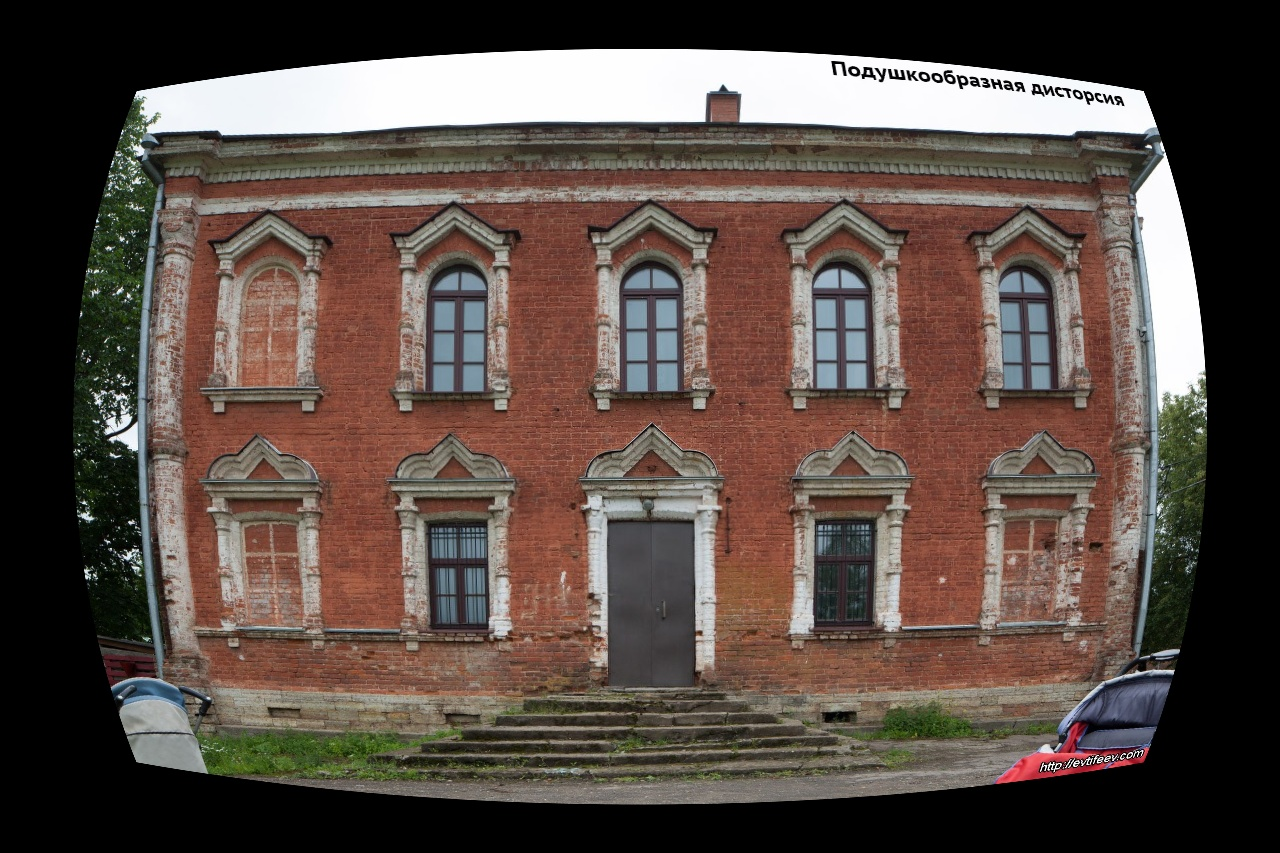
\includegraphics[scale=0.4]{../images/results/after_bd_applied_img.jpg}
    \caption{Изображение после применения бочкообразной дисторсии}
\end{figure}
\newpage
\noindent Как можно заметить, мы хоть и получили области с неопределенной интесивностью по краям изображения, геометрических искажений стало меньше и дом выглядит действительно прямоугольным, что и было целью преобразования. С получившейся черной <<рамкой>> можно бороться с помощью геом.преобразований.

\noindent Перейдем к коррекции бочкообразной дисторсии.
\\
\noindent \textbf{Листинг 3.2} Наложение подушкообразной дисторсии
\begin{lstlisting}
cv::Mat pincushion_distortion(cv::Mat img) {
    cv::Mat xi, yi;
    std::vector<float> t_x, t_y;
    for (int i = 0; i < img.cols; i++) {
        t_x.push_back(float(i));
    } 
    for (int i = 0; i < img.rows; i++) {
        t_y.push_back(float(i));
    }

    cv::repeat(cv::Mat(t_x).reshape(1, 1), img.rows, 1, xi);
    cv::repeat(cv::Mat(t_y).reshape(1, 1).t(), 1, img.cols, yi);

    double xmid = xi.cols / 2.0;
    double ymid = xi.rows / 2.0;
    xi -= xmid;
    xi /= xmid;
    yi -= ymid;
    yi /= ymid;

    cv::Mat r, theta;
    cv::cartToPolar(xi, yi, r, theta);
    double F3(-0.2);
    cv::Mat r2;

    cv::pow(r, 2, r2);
    r += r2 * F3;

    cv::Mat u, v;
    cv::polarToCart(r, theta, u, v);
    u *= xmid;
    u += xmid;
    v *= ymid;
    v += ymid;

    cv::Mat img_pincushion;
    cv::remap(img, img_pincushion, u, v, cv::INTER_LINEAR);
    return img_pincushion;
}
\end{lstlisting}

\begin{figure}[h]
    \centering
    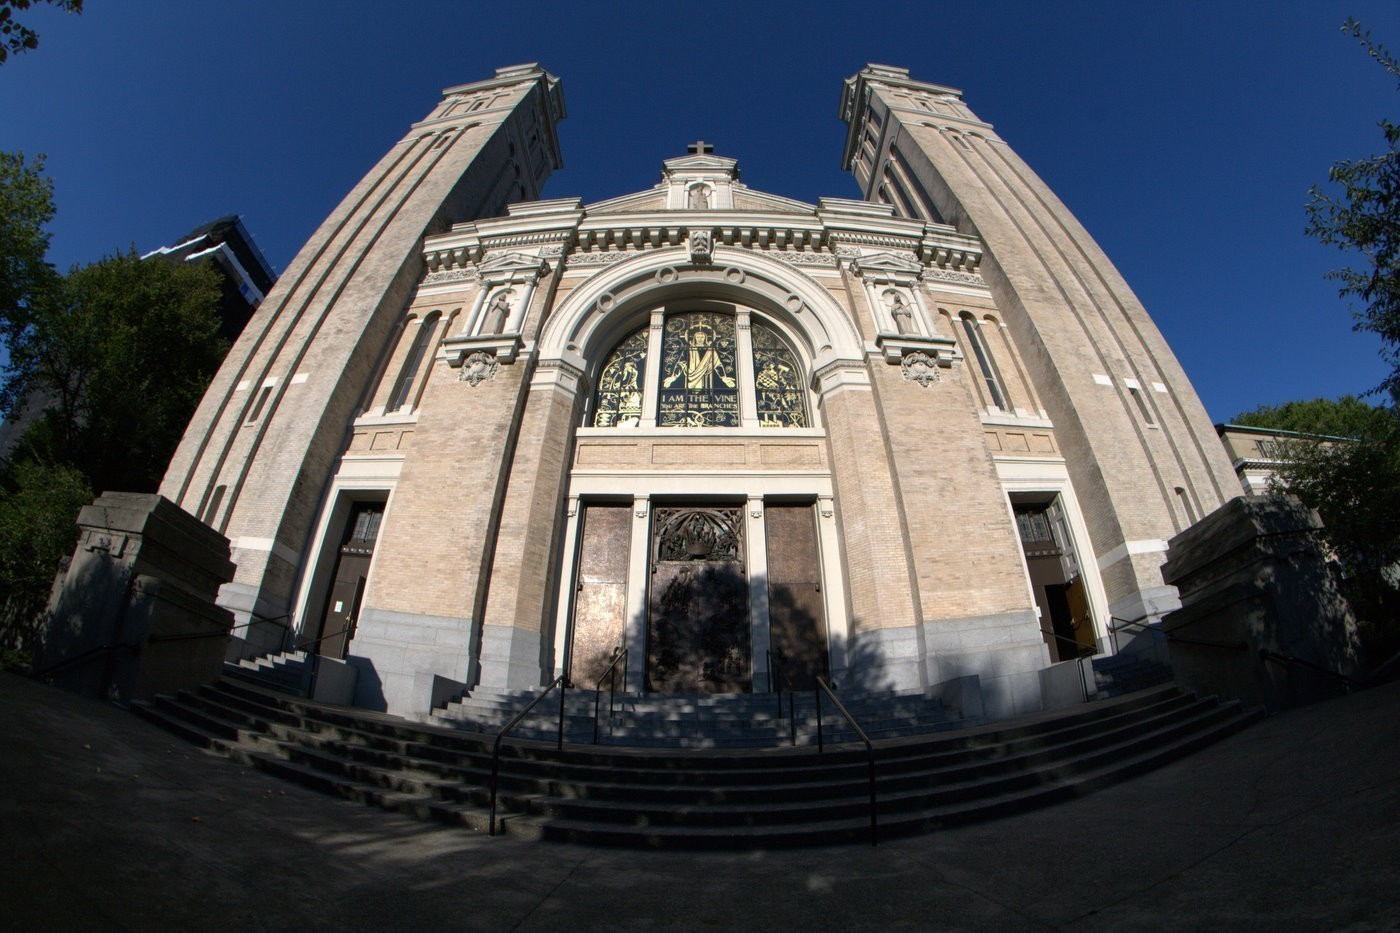
\includegraphics[scale=0.3]{../images/original/bd.jpg}
    \caption{Изображение с выраженной бочкообразной дисторсией}
\end{figure}
\begin{figure}[h]
    \centering
    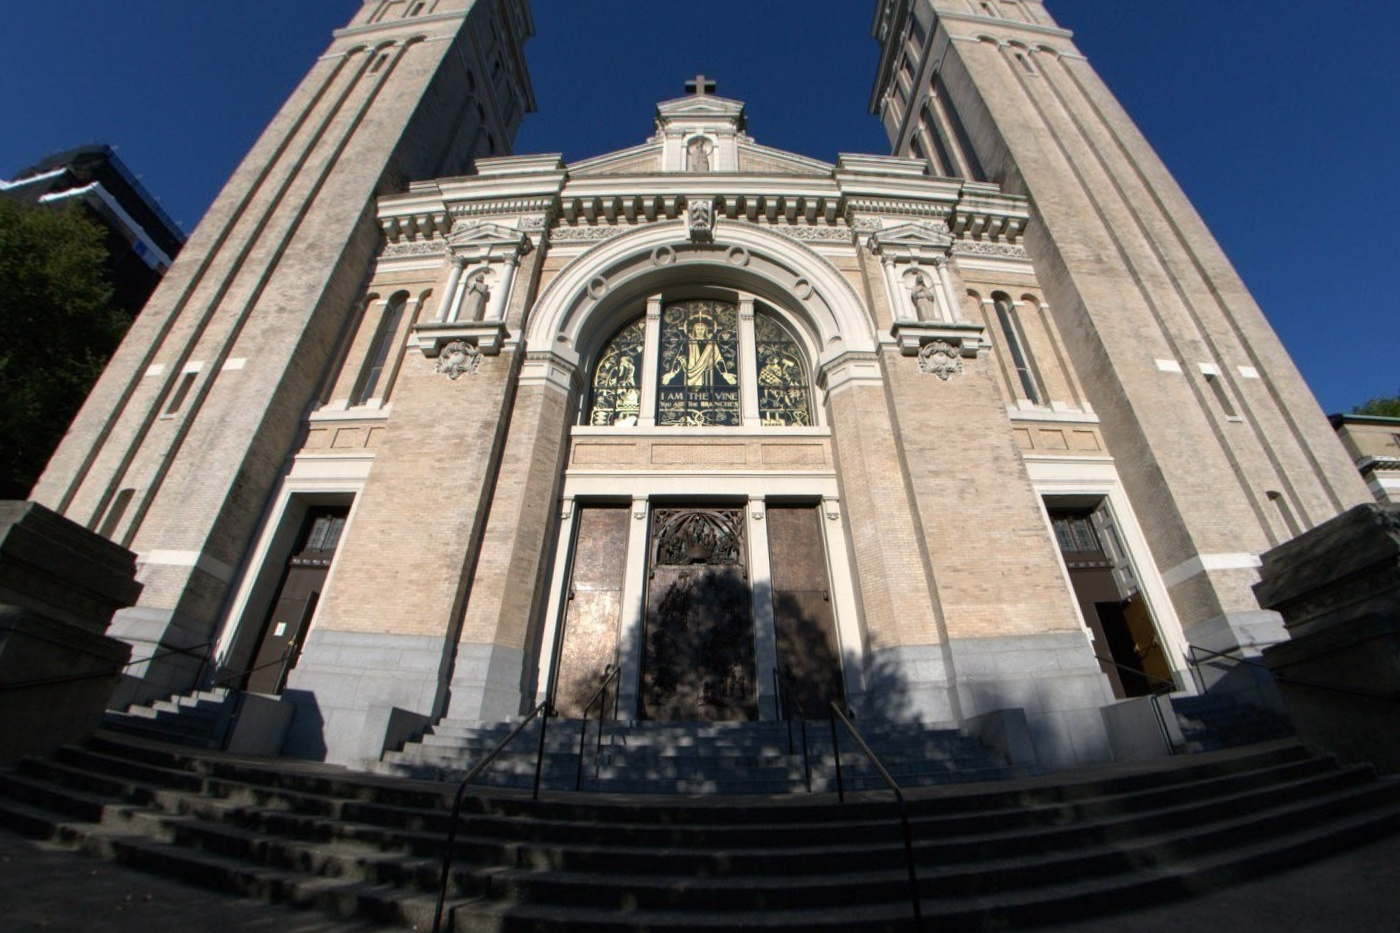
\includegraphics[scale= 0.3 ]{../images/results/after_pd_applied_img.jpg}
    \caption{Изображение после наложения подушкообразной дисторсии}
\end{figure}
\noindent Заметим, что наложение подушкообразной дисторсии действительно помогло выровнять изображение.
Но, с другой стороны, привело к небольшим потерям данных по краям изображения. Неидельно, но и неудивительно, конечно.
\newpage

\section{<<Склейка>> изображений}
\subsection{Ручная склейка изображений }
\begin{figure}[h]
    \centering
    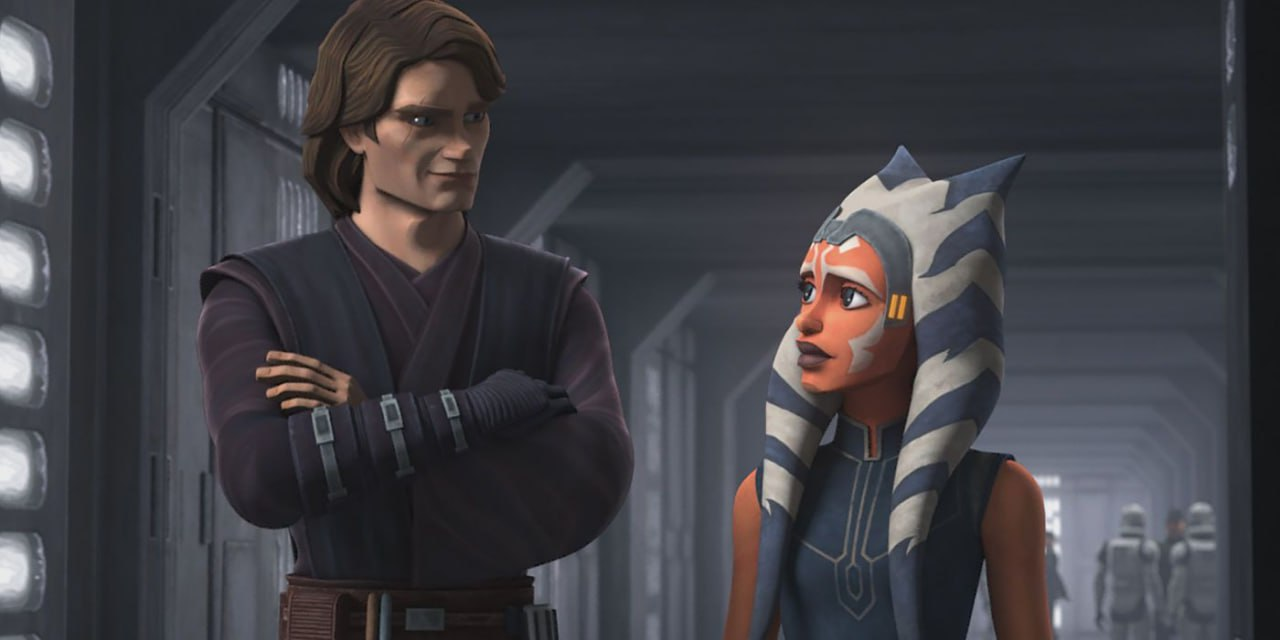
\includegraphics[scale= 0.55]{../images/original/img_to_be_cut_and_glued.jpeg}
    \caption{Исходное изображение}
\end{figure}
\begin{figure}[h]
    \centering
    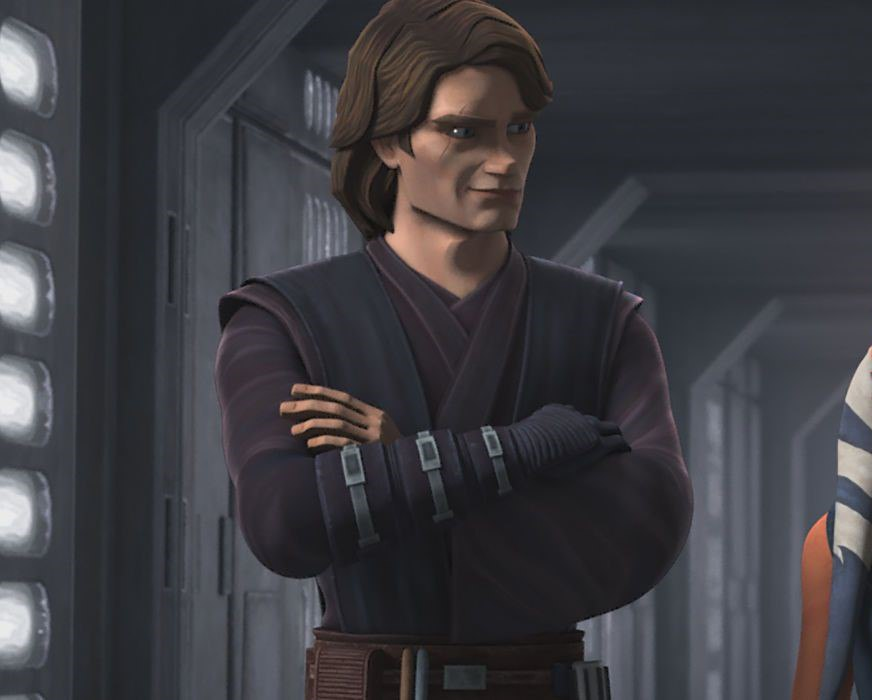
\includegraphics[scale= 0.3 ]{../images/original/glue_part_1}
    \caption{Левая часть изображения}
\end{figure}

\begin{figure}[h]
    \centering
    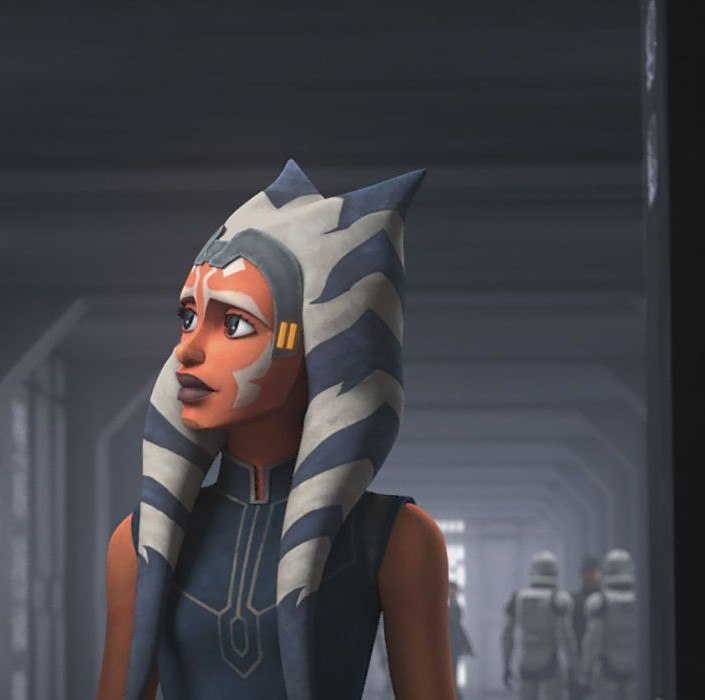
\includegraphics[scale= 0.3]{../images/original/glue_part_2.jpeg}
    \caption{Правая часть изображения}
\end{figure}
\newpage
\noindent \textbf{Листинг 4.1} Ручная склейка изображений
\begin{lstlisting}
cv::Mat glue_images(cv::Mat left_part, cv::Mat right_part) {
	int templ_size = 20;
	cv::Mat templ = left_part(cv::Rect(left_part.cols - templ_size - 1, 0, templ_size, left_part.rows));
	
	cv::Mat res;
	cv::matchTemplate(right_part, templ, res, cv::TM_CCOEFF);
	double min_val, max_val;
	cv::Point2i min_loc, max_loc;
	cv::minMaxLoc(res, &min_val, &max_val, &min_loc, &max_loc);
	cv::Mat final_img = cv::Mat::zeros(left_part.rows, left_part.cols + right_part.cols - max_loc.x - templ_size, left_part.type());
	left_part.copyTo(final_img(cv::Rect(0, 0, left_part.cols, left_part.rows)));
	cv::Mat right_part_for_glue = right_part(cv::Rect(max_loc.x + templ_size, 0, right_part.cols - max_loc.x - templ_size, right_part.rows));
	right_part_for_glue.copyTo(final_img(cv::Rect(left_part.cols, 0, right_part.cols - max_loc.x - templ_size, right_part.rows)));
	return final_img;
}
\end{lstlisting}
\newpage
\begin{figure}[h]
    \centering
   
    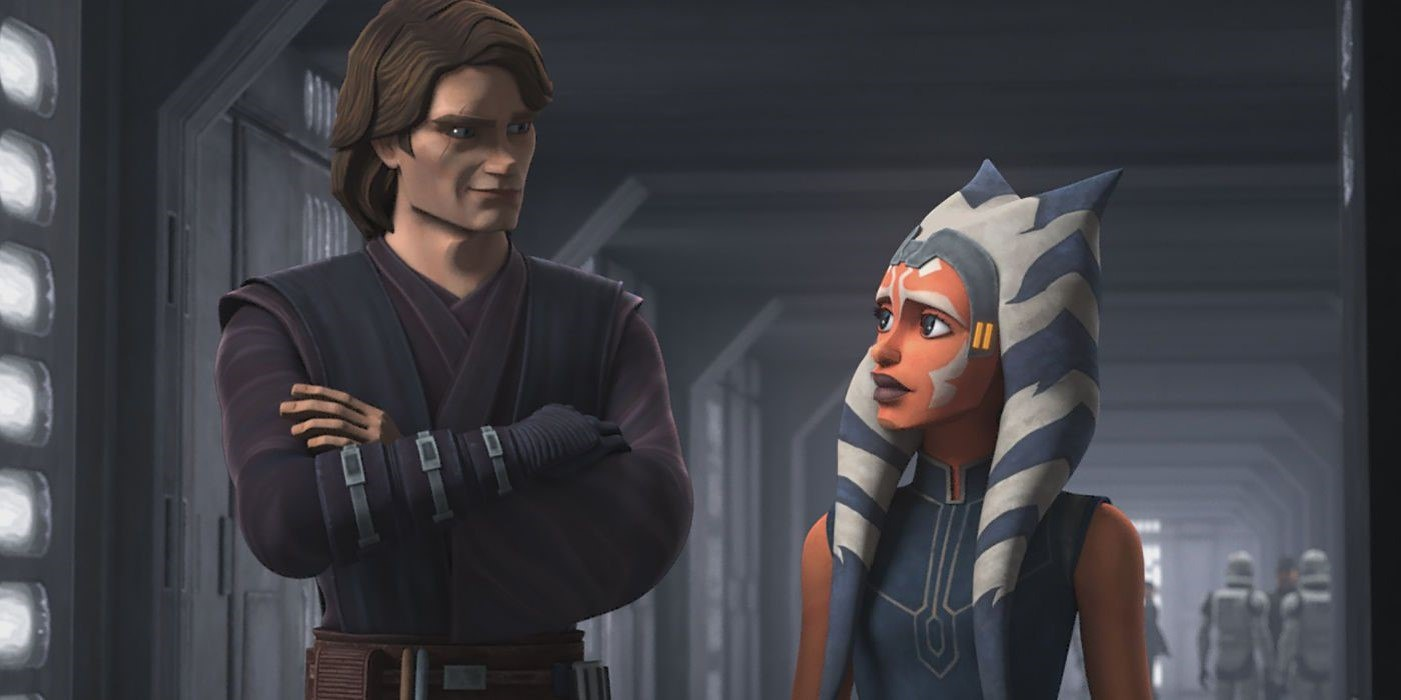
\includegraphics[scale=0.4]{../images/results/manually_glued_img.jpeg}
    \caption{Склеенное изображение}
\end{figure}
\noindent По сути, метод  работает за счет приведения одной части в систему координат другой части изображения. Скейлка получилась достаточно незаметной, в том числе за счет аккуратно угаданного параметра templ\_size.

\subsection{Автоматическая склейка в OpenCV}
\noindent А вот автоматическая скейка лажает (либо я в что-то сделал не так, тоже вариант), но склеить конкретно эти два изоюбражения не вышло, возможно, потому что общих точек на них маловато.
\\ \noindent \textbf{Листинг 4.2} Автоматическая склейка в opencv
\begin{lstlisting}
cv::Mat auto_glue_images(cv::Mat left_part, cv::Mat right_part) {
	cv::Ptr<cv::Stitcher> stitcher = cv::Stitcher::create(cv::Stitcher::PANORAMA);
	std::vector<cv::Mat> imgs;
	imgs.push_back(left_part);
	imgs.push_back(right_part);
	cv::Mat img_stitched;
	cv::Stitcher::Status status = stitcher->stitch(imgs, img_stitched);
	return img_stitched;
}

\end{lstlisting}

\newpage
\section{Заключение}
\noindent \textbf{Выводы: } я применил несколько отобржений и геометрических преобразований для решения задач пространственной коррекции изоображений.
Опять немножко позже дедлайна, но и третья лаба почти-почти готова, так что шансы нагнать как никогда велики. <<Долго запрягаем, да быстро едем>>, дааа....
\\ \textbf{Ответы на вопросы после лабораторной работы: } 
\begin{enumerate}
    \item Можно отразить относительно оси Ox - эквивалетно повороту на 180. Хотя фактически такая матрица отражения - лишь частный случай матрицы поворота; 
    \item В соответствии с формулой $t_{min} = \frac{(n+1)(n+2)}{2} = 15$ точек;
    \item Связано с тем что область, содержащая информацию о нашем изображении меняеет местоположение относительно исходного <<холста>>. Что неизбежно приводит к появлению полностью черных областей. Можно бороться с этим с помощью дополнительного масштабирования изображения.
\end{enumerate}
\end{document}
 